% Options for packages loaded elsewhere
\PassOptionsToPackage{unicode}{hyperref}
\PassOptionsToPackage{hyphens}{url}
\PassOptionsToPackage{dvipsnames,svgnames*,x11names*}{xcolor}
%
\documentclass[
]{article}
\usepackage{amsmath,amssymb}
\usepackage{lmodern}
\usepackage{iftex}
\ifPDFTeX
  \usepackage[T1]{fontenc}
  \usepackage[utf8]{inputenc}
  \usepackage{textcomp} % provide euro and other symbols
\else % if luatex or xetex
  \usepackage{unicode-math}
  \defaultfontfeatures{Scale=MatchLowercase}
  \defaultfontfeatures[\rmfamily]{Ligatures=TeX,Scale=1}
\fi
% Use upquote if available, for straight quotes in verbatim environments
\IfFileExists{upquote.sty}{\usepackage{upquote}}{}
\IfFileExists{microtype.sty}{% use microtype if available
  \usepackage[]{microtype}
  \UseMicrotypeSet[protrusion]{basicmath} % disable protrusion for tt fonts
}{}
\makeatletter
\@ifundefined{KOMAClassName}{% if non-KOMA class
  \IfFileExists{parskip.sty}{%
    \usepackage{parskip}
  }{% else
    \setlength{\parindent}{0pt}
    \setlength{\parskip}{6pt plus 2pt minus 1pt}}
}{% if KOMA class
  \KOMAoptions{parskip=half}}
\makeatother
\usepackage{xcolor}
\IfFileExists{xurl.sty}{\usepackage{xurl}}{} % add URL line breaks if available
\IfFileExists{bookmark.sty}{\usepackage{bookmark}}{\usepackage{hyperref}}
\hypersetup{
  pdftitle={RIBBiTR Schema's},
  colorlinks=true,
  linkcolor={Maroon},
  filecolor={Maroon},
  citecolor={Blue},
  urlcolor={blue},
  pdfcreator={LaTeX via pandoc}}
\urlstyle{same} % disable monospaced font for URLs
\usepackage[margin=1in]{geometry}
\usepackage{graphicx}
\makeatletter
\def\maxwidth{\ifdim\Gin@nat@width>\linewidth\linewidth\else\Gin@nat@width\fi}
\def\maxheight{\ifdim\Gin@nat@height>\textheight\textheight\else\Gin@nat@height\fi}
\makeatother
% Scale images if necessary, so that they will not overflow the page
% margins by default, and it is still possible to overwrite the defaults
% using explicit options in \includegraphics[width, height, ...]{}
\setkeys{Gin}{width=\maxwidth,height=\maxheight,keepaspectratio}
% Set default figure placement to htbp
\makeatletter
\def\fps@figure{htbp}
\makeatother
\setlength{\emergencystretch}{3em} % prevent overfull lines
\providecommand{\tightlist}{%
  \setlength{\itemsep}{0pt}\setlength{\parskip}{0pt}}
\setcounter{secnumdepth}{-\maxdimen} % remove section numbering
\ifLuaTeX
  \usepackage{selnolig}  % disable illegal ligatures
\fi

\title{RIBBiTR Schema's}
\author{}
\date{\vspace{-2.5em}Updated: 2022-11-07}

\begin{document}
\maketitle

\hypertarget{data-acquisition-protocol}{%
\subsection{Data Acquisition Protocol}\label{data-acquisition-protocol}}

\begin{itemize}
\tightlist
\item
  Select variables of interest from the data tables within schemas
\item
  Contact data owners within RIBBiTR for approved use of data; CC data
  manager

  \begin{itemize}
  \tightlist
  \item
    Per
    \href{https://docs.google.com/document/d/1m1EEuUH3ioVVXtFkDaWFHITddPcmputEhZxfW_omtrI/edit\#heading=h.q4aj1repk7gi}{RIBBiTR
    data sharing agreement}
  \item
    Data owners

    \begin{itemize}
    \tightlist
    \item
      Panama Survey Data: \href{jvoyles@unr.edu}{Jamie Voyles}
    \item
      SERDP Survey Data: \href{cori.zawacki@pitt.edu}{Cori
      Richards-Zawacki}
    \item
      Pennsylvania Survey Data: \href{cori.zawacki@pitt.edu}{Cori
      Richards-Zawacki}
    \item
      Sierra Nevada Survey Data: \href{roland.knapp@ucsb.edu}{Roland
      Knapp}
    \item
      Brazil Legacy Survey Data: \href{guibecker@psu.edu}{Gui Becker}
    \item
      AMP: \href{louise.rollins-smith@vanderbilt.edu}{Louise
      Rollins-Smith}
    \item
      Microbiome: \href{dwoodhams@gmail.com}{Doug Woodhams}
    \item
      Genetic: \href{rosenblum@berkeley.edu}{Bree Rosenblum}
    \item
      Antibody: \href{louise.rollins-smith@vanderbilt.edu}{Louise
      Rollins-Smith}
    \item
      Bacterial: \href{dwoodhams@gmail.com}{Doug Woodhams}
    \item
      Mucosome: \href{dwoodhams@gmail.com}{Doug Woodhams}
    \end{itemize}
  \end{itemize}
\item
  Contact data manager to develop query for variables of interest
\item
  \emph{Note}: If you are requesting data from a processed swab table,
  then you must also contact the team that collected the swab and the
  team that processed the swab.
\end{itemize}

\hypertarget{swab-data-nomenclature}{%
\subsection{Swab Data Nomenclature}\label{swab-data-nomenclature}}

\begin{itemize}
\tightlist
\item
  bd\_swab\_id: dry swab used for Bd detection
\item
  genetic\_id: sample used for genetic processing (buccal, toe clip,
  tissue)
\item
  bacterial\_swab\_id: swab used for culturing bacteria
\item
  mucosome\_id: sample used for identifying all micro organisms
\item
  microbiome\_swab\_id: swab used for sequencing bacteria
\item
  crispr\_swab\_id: swab used for crispr Bd detection
\item
  amp\_id: sample used for anti-microbial peptide processing
\item
  antibody\_id:
\end{itemize}


\includegraphics[width=1.82292in,height=\textheight]{ribbitr.png}

\includegraphics[width=1.04167in,height=\textheight]{nsf_logo.png}

\hypertarget{schema-survey_data}{%
\subsection{Schema: ``survey\_data''}\label{schema-survey_data}}

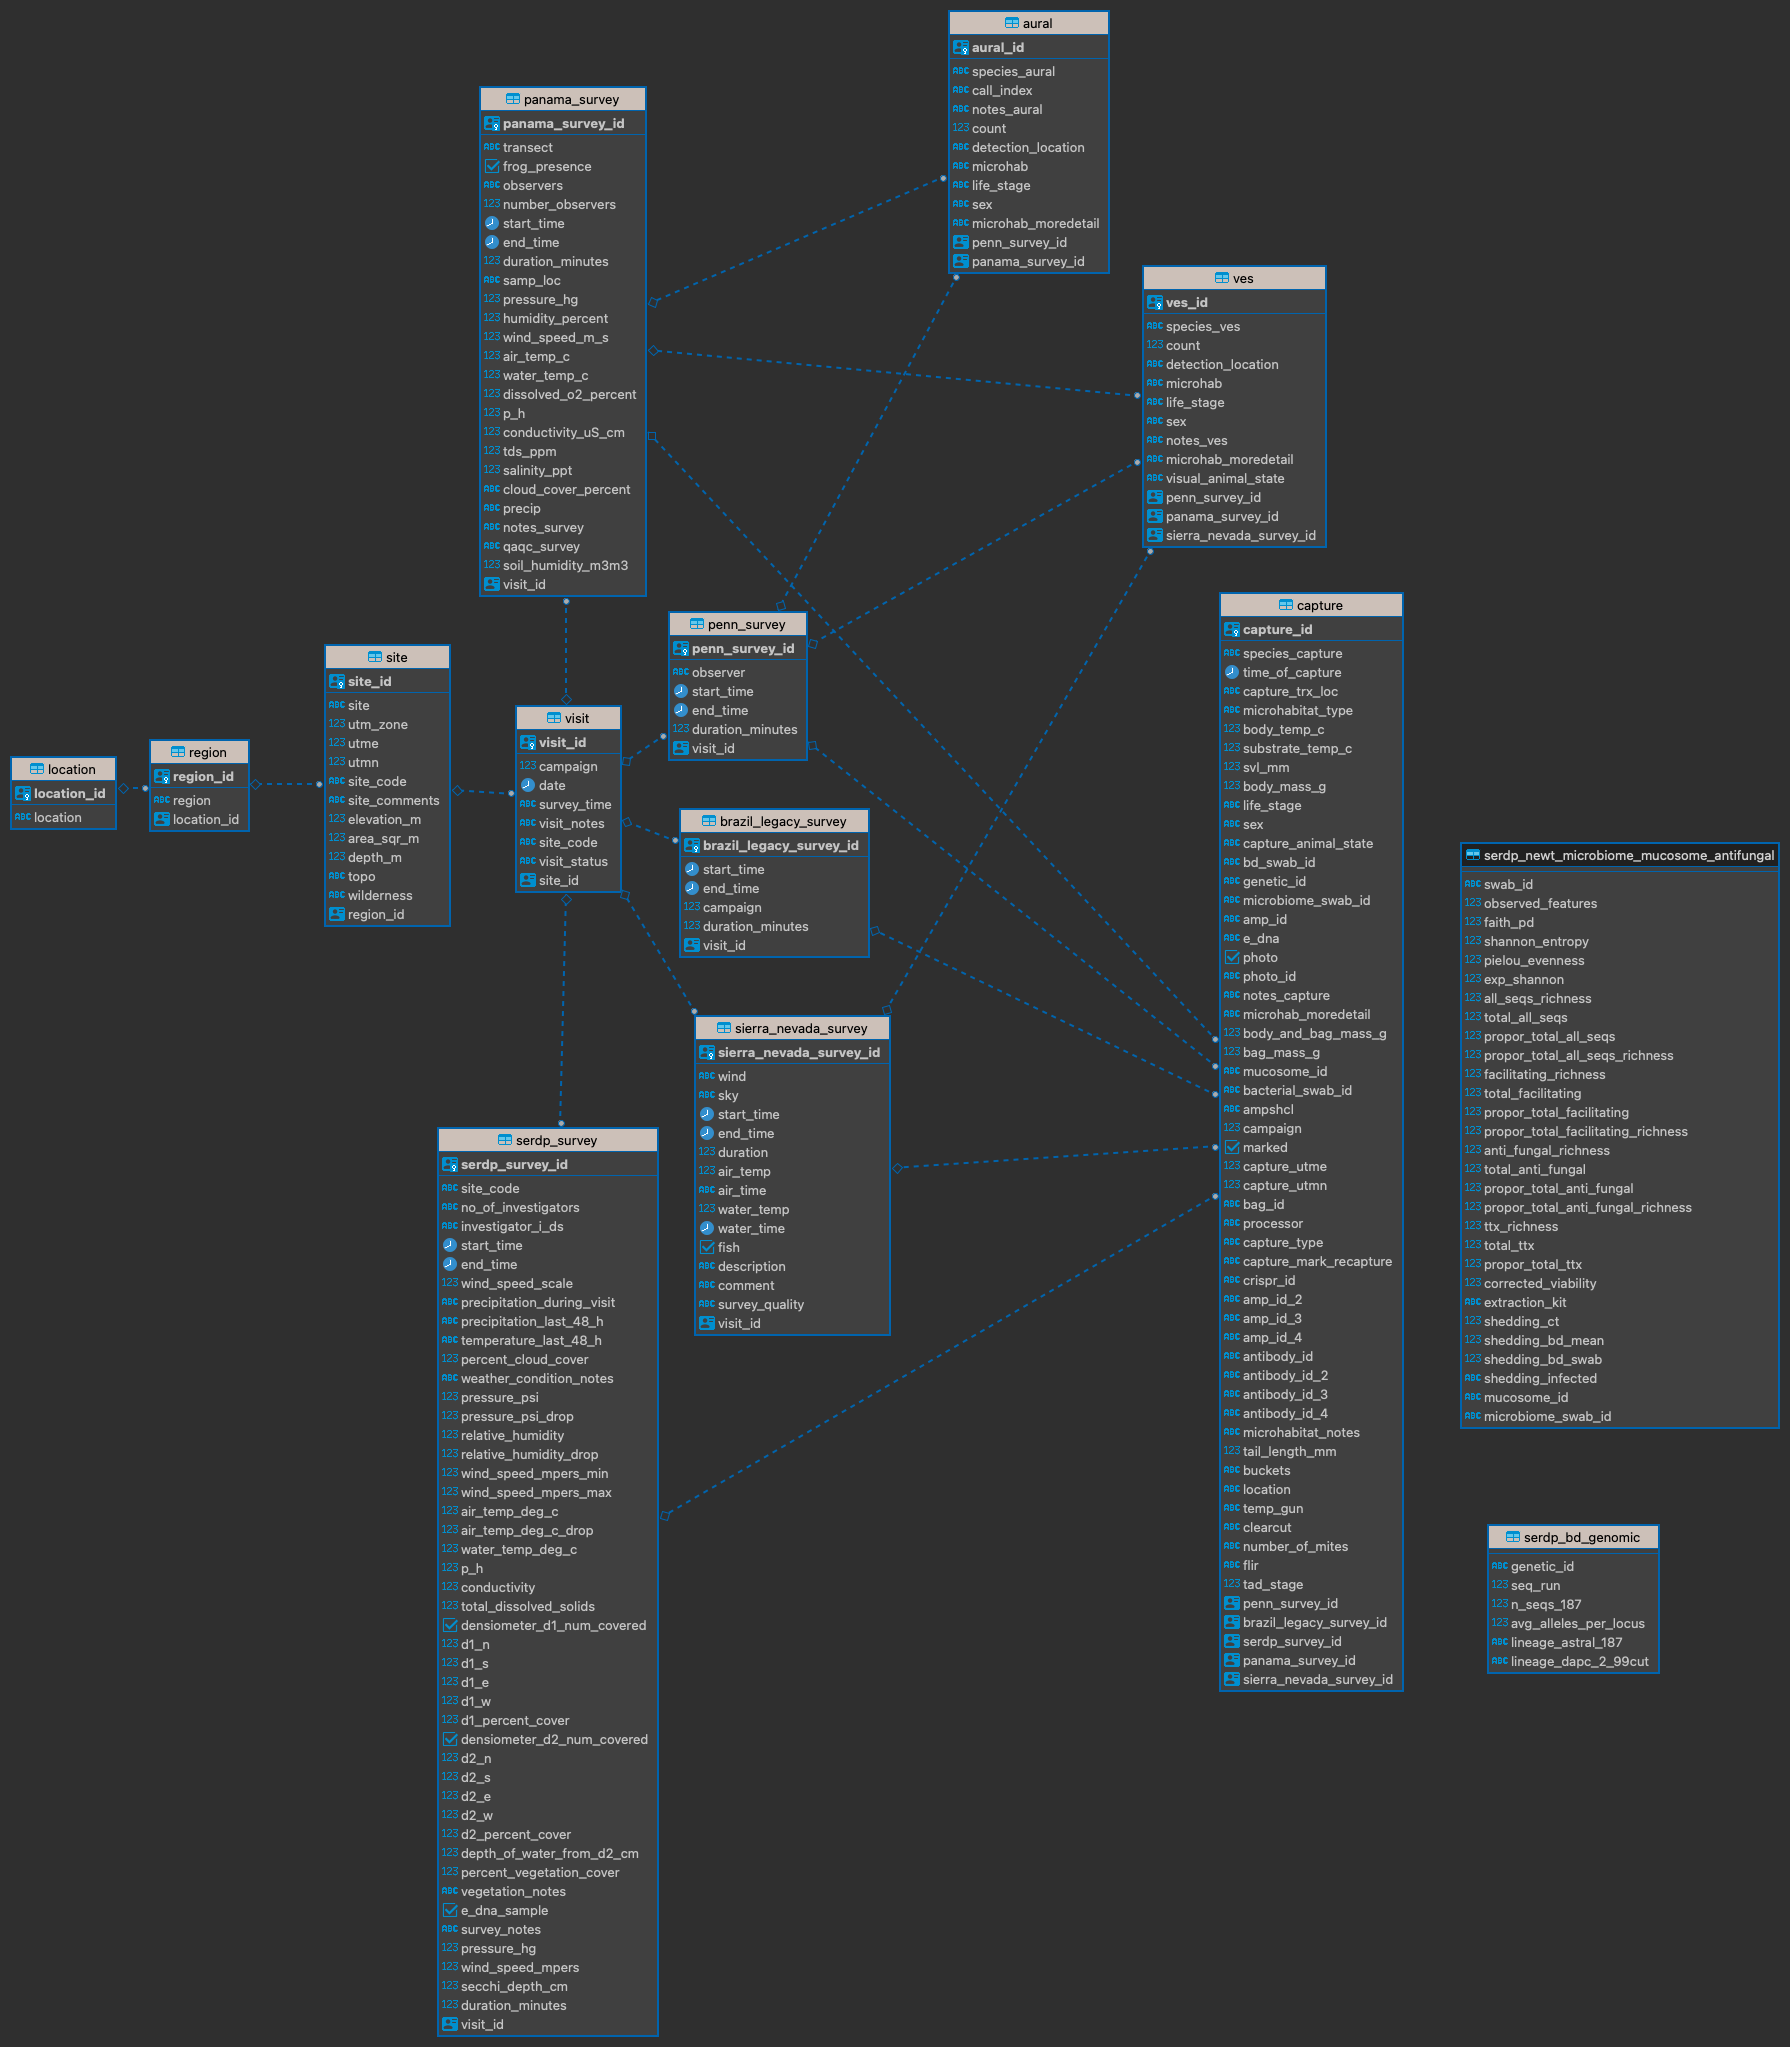
\includegraphics{RIBBiTR - survey_data.png}

\hypertarget{schema-hobo}{%
\subsection{Schema: ``hobo''}\label{schema-hobo}}

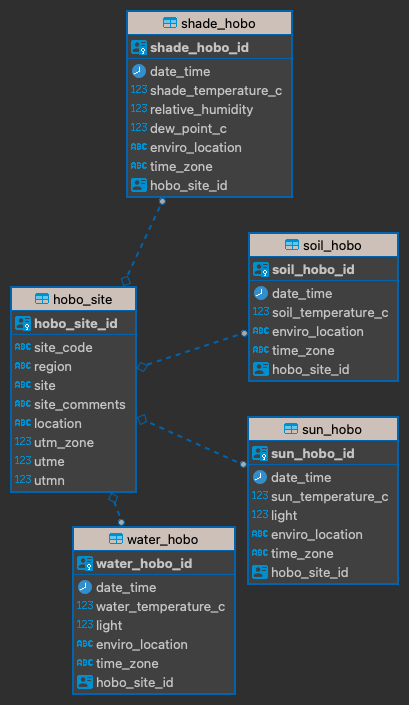
\includegraphics{RIBBiTR - hobo.png}

\hypertarget{schema-antifungal_isolate}{%
\subsection{Schema:
``antifungal\_isolate''}\label{schema-antifungal_isolate}}

\includegraphics{RIBBiTR - antifungal_isolate_ref.png}

\end{document}
